%% FigCubicTernary Complex Model Homodimer Tree
%% FigS2CubicTernaryComplexHomodimerTree.tex
%% Unused packages and definitions removed; TikZ/PGFPlots source formatted.

\documentclass{standalone}

\usepackage{tikz}
\usetikzlibrary{arrows}

\def\half{\frac{1}{2}}
\def\e{\mathsf{e}}

\def\kappae#1{\kappa_{\e_#1}}

\begin{document}

\tikzstyle{every node}=[outer sep=1pt,inner sep=1pt]
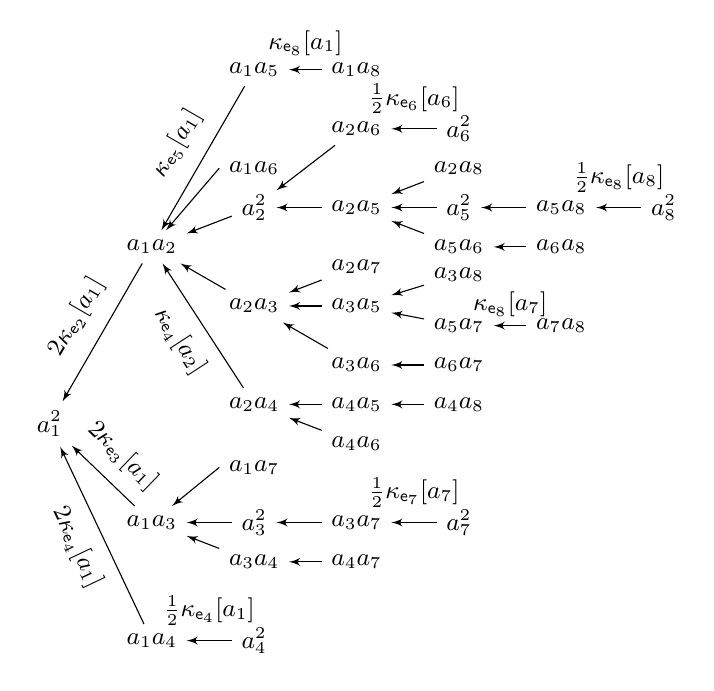
\begin{tikzpicture}[>=latex',font=\small,node distance=1.3cm]

    \draw (-10,3) node (AA) {$a_1^2$};

    \node[right of=AA,yshift=2.25cm] (AB) {$a_1a_2$};
    \draw[<-] (AA) to node[above,sloped,yshift=3pt] {$2\kappae{2}[a_1]$} (AB);

    \node[right of=AA,yshift=-1.25cm] (AC) {$a_1a_3$};
    \draw[<-] (AA) to node[sloped,above,yshift=2pt] {$2\kappae{3}[a_1]$} (AC);

    \node[right of=AA,yshift=-2.75cm] (AD) {$a_1a_4$};
    \draw[<-] (AA) to node[sloped,below,yshift=-2pt] {$2\kappae{4}[a_1]$} (AD);

    \node[right of=AB,yshift=2.25cm] (AE) {$a_1a_5$};
    \draw[<-] (AB) to node[above,sloped,yshift=3pt] {$\kappae{5}[a_1]$} (AE);

    \node[right of=AB,yshift=0.5cm] (BB) {$a_2^2$};
    \draw[<-] (AB) to (BB);

    \node[right of=AB,yshift=-0.75cm] (BC) {$a_2 a_3 $};
    \draw[<-] (AB) to (BC);

    \node[right of=AC] (CC) {$a_3^2$};
    \draw[<-] (AC) to (CC);

    \node[right of=AB,yshift=-2cm] (BD) {$a_2 a_4$};
    \draw[<-] (AB) to node[sloped,below,yshift=-2pt] {$\kappae{4}[a_2]$} (BD);

    \node[right of=AC,yshift=-0.5cm] (CD) {$a_3 a_4$};
    \draw[<-] (AC) to (CD);

    \node[right of=AD] (DD) {$a_4^2$};
    \draw[<-] (AD) to node[above,yshift=2pt] {$\half \kappae{4}[a_1]$} (DD);

    \node[right of=BB] (BE) {$a_2 a_5$};
    \draw[<-] (BB) to (BE);

    \node[right of=BC] (CE) {$a_3 a_5$};
    \draw[<-] (BC) to (CE);

    \node[right of=BD,yshift=0cm] (DE) {$a_4 a_5 $};
    \draw[<-] (BD) to (DE);

    \node[right of=BE] (EE) {$a_5^2$};
    \draw[<-] (BE) to (EE);

    \node[right of=AB,yshift=1cm] (AF) {$a_1a_6$};
    \draw[<-] (AB) to (AF.west);

    \node[right of=BB,yshift=1cm] (BF) {$a_2 a_6$};
    \draw[<-] (BB) to   (BF);

    \node[right of=BC,yshift=-0.75cm] (CF) {$a_3 a_6$};
    \draw[<-] (BC) to (CF);

    \node[right of=BD,yshift=-0.5cm] (DF) {$a_4 a_6 $};
    \draw[<-] (BD) to (DF);

    \node[right of=BE,yshift=-0.5cm] (EF) {$a_5 a_6 $};
    \draw[<-] (BE) to (EF);

    \node[right of=BF,yshift=0cm] (FF) {$a_6^2$};
    \draw[<-] (BF) to node[sloped,above,yshift=2pt] {$\half \kappae{6}[a_6]$} (FF);

    \node[right of=AC,yshift=0.7cm] (AG) {$a_1a_7$};
    \draw[<-] (AC) to (AG.west);

    \node[right of=BC,yshift=0.5cm] (BG) {$a_2 a_7$};
    \draw[<-] (BC) to (BG);

    \node[right of=CC] (CG) {$a_3 a_7$};
    \draw[<-] (CC) to   (CG);

    \node[right of=CD] (DG) {$a_4 a_7$};
    \draw[<-] (CD) to (DG);

    \node[right of=CE,yshift=-0.25cm] (EG) {$a_5 a_7$};
    \draw[<-] (CE) to (EG);

    \node[right of=BE,yshift=0.5cm] (BH) {$a_2 a_8$};
    \draw[<-] (BE) to (BH);

    \node[right of=CE,yshift=0.4cm] (CH) {$a_3 a_8$};
    \draw[<-] (CE) to (CH);

    \node[right of=DE] (DH) {$a_4 a_8$};
    \draw[<-] (DE) to (DH);

    \node[right of=CF] (FG) {$a_6 a_7$};
    \draw[<-] (CF) to (FG);

    \node[right of=CG] (GG) {$a_7^2$};
    \draw[<-] (CG) to node[above,yshift=2pt] {$\half\kappae{7}[a_7]$} (GG);

    \node[right of=AE] (AH) {$a_1a_8$};
    \draw[<-] (AE) to node[above,yshift=4pt,inner sep=1pt] {$\kappae{8}[a_1]$} (AH);

    \node[right of=EE] (EH) {$a_5 a_8$};
    \draw[<-] (EE) to (EH);

    \node[right of=EF] (FH) {$a_6 a_8$};
    \draw[<-] (EF) to  (FH);

    \node[right of=EG] (GH) {$a_7 a_8$};
    \draw[<-] (EG) to  node[above,yshift=2pt,inner sep=1pt] {$\kappae{8}[a_7]$}(GH);

    \node[right of=EH] (HH) {$a_8^2$};
    \draw[<-] (EH) to node[above,yshift=2pt] {$\half \kappae{8}[a_8]$} (HH);

\end{tikzpicture}

\end{document}

